% Informe: Implementación y Análisis de Complejidad de Listas, Pilas y Colas en Java
% Compilar con XeLaTeX (dos pasadas):   cd informe && xelatex informe.tex && xelatex informe.tex
% Las tablas (tablas/*.tex) y figuras (figuras/*.pdf) las genera analisis/graficar.py

\documentclass[11pt,a4paper]{article}

% ---------------------------------------------------------------------------
% Datos del estudiante (EDITAR AQUÍ)
% ---------------------------------------------------------------------------
\newcommand{\estudiante}{Brallan Esteban Ardila Osorio}
\newcommand{\codigo}{1140915162}
\newcommand{\correo}{bardilao@unal.edu.co}
\newcommand{\repositorio}{https://github.com/BrayanARDL/Laboratorio-stack-queue-java-ed-}

% ---------------------------------------------------------------------------
\usepackage{fontspec}
\usepackage{polyglossia}
\setdefaultlanguage{spanish}
\usepackage[margin=2.3cm]{geometry}
\usepackage{graphicx}
\usepackage{booktabs}
\usepackage{float}
\usepackage[font=small,labelfont=bf]{caption}
\usepackage{amsmath}
\usepackage{xcolor}
\usepackage{listings}
\usepackage{enumitem}
\usepackage{multirow}
\usepackage{array}
\usepackage{tabularx}
\usepackage[hidelinks]{hyperref}

\setmainfont{Latin Modern Roman}
\setmonofont{DejaVu Sans Mono}[Scale=0.82]

\definecolor{azul}{HTML}{2a78d6}
\definecolor{gris}{HTML}{52514e}
\definecolor{fondo}{HTML}{f5f5f3}
\hypersetup{colorlinks=true, linkcolor=azul, urlcolor=azul, citecolor=azul}

\lstset{
  language=Java, basicstyle=\ttfamily\small, backgroundcolor=\color{fondo},
  keywordstyle=\color{azul}\bfseries, commentstyle=\color{gris}\itshape,
  frame=single, rulecolor=\color{fondo}, framesep=4pt, xleftmargin=6pt, xrightmargin=6pt,
  showstringspaces=false, columns=fullflexible, keepspaces=true, breaklines=true,
  aboveskip=6pt, belowskip=6pt
}
\setlist{itemsep=2pt, topsep=4pt}
\setlength{\emergencystretch}{3em}   % evita líneas desbordadas por palabras en \texttt
\renewcommand{\arraystretch}{1.12}
\newcommand{\us}{\,µs}
\newcommand{\Oone}{$O(1)$}
\newcommand{\On}{$O(n)$}

% Tabla de tiempos a ancho completo
\newcommand{\tablatiempos}[2]{%
  \begin{table}[H]\centering\small
  \caption{#2}
  \resizebox{\linewidth}{!}{\input{tablas/#1}}
  \end{table}}
% Tabla de tiempos con pocas columnas: tamaño natural
\newcommand{\tablatiemposcorta}[2]{%
  \begin{table}[H]\centering\small
  \caption{#2}
  \input{tablas/#1}
  \end{table}}

\begin{document}

% ===========================================================================
% PORTADA
% ===========================================================================
\begin{titlepage}
\centering
\vspace*{1.5cm}
{\large Universidad Nacional de Colombia\par}
{\large Estructuras de Datos --- 2026-2\par}
\vspace{2.8cm}
{\LARGE\bfseries Implementación y Análisis de Complejidad\\[4pt] de Listas, Pilas y Colas en Java\par}
\vspace{0.8cm}
\vspace{3cm}
{\large \estudiante\par}
{\normalsize \codigo\ \textperiodcentered\ \correo\par}
\vspace{1.6cm}
{\normalsize Profesor: David Herrera\par}
{\normalsize Monitora: Ángela Camila Siabato Londoño\par}
\vfill
{\normalsize Repositorio: \url{\repositorio}\par}
\vspace{0.4cm}
{\normalsize Septiembre de 2026\par}
\end{titlepage}

\tableofcontents
\newpage

% ===========================================================================
\section{Objetivo}
% ===========================================================================
Implementar en Java, sin usar las colecciones de la librería estándar, la estructura \textbf{List} con
listas enlazadas en cuatro variantes (simplemente enlazada sin cola y con cola, doblemente enlazada sin
cola y con cola) y las estructuras \textbf{MyStack} (pila) y \textbf{MyQueue} (cola) sobre un
\textbf{arreglo circular dinámico}. Luego, analizar la complejidad de cada método de dos formas:
\emph{teóricamente}, con notación Big-O, y \emph{empíricamente}, midiendo tiempos de ejecución con
tamaños de $10^1$ a $10^8$ elementos. Con ambos análisis se comparan las implementaciones entre sí y
se sacan conclusiones sobre cuándo conviene cada una.

El código fuente, los datos crudos de las mediciones y los scripts para reproducir todo están en el
repositorio: \url{\repositorio}.

% ===========================================================================
\section{Explicación de la implementación}
% ===========================================================================

\subsection{Organización del código}

\begin{table}[H]\centering\small
\begin{tabularx}{\linewidth}{>{\ttfamily}l X}
\toprule
\normalfont\textbf{Paquete / archivo} & \textbf{Contenido} \\
\midrule
listas/LinkedListADT & Interfaz común de las cuatro listas (\texttt{pushFront}, \texttt{pushBack}, \texttt{popFront}, \texttt{popBack}, \texttt{topFront}, \texttt{topBack}, \texttt{find}, \texttt{erase}, \texttt{addBefore}, \texttt{addAfter}, \texttt{isEmpty}, \texttt{size}). \\
listas/SNode, DNode & Nodo simple (\texttt{key}, \texttt{next}) y nodo doble (\texttt{key}, \texttt{next}, \texttt{prev}). \\
listas/* & \texttt{SinglyLinkedList}, \texttt{SinglyLinkedListTail}, \texttt{DoublyLinkedList}, \texttt{DoublyLinkedListTail}. \\
pilacola/MyStack, MyQueue & Interfaces pedidas en el enunciado. \\
pilacola/CircularDynamicArray & Arreglo circular que crece duplicando su capacidad; es la base común. \\
pilacola/ArrayStack, ArrayQueue & Implementaciones de \texttt{MyStack} y \texttt{MyQueue} sobre el arreglo circular. \\
pruebas/Pruebas & Pruebas de correctitud (no miden tiempo). \\
benchmark/Benchmark & Medición de tiempos; escribe \texttt{resultados/tiempos.csv}. \\
analisis/graficar.py & Lee el CSV y genera las gráficas y tablas de este informe. \\
\bottomrule
\end{tabularx}
\end{table}

Las cuatro listas implementan la misma interfaz genérica \texttt{LinkedListADT<T, N>}, donde \texttt{N}
es el tipo de nodo. Así el benchmark usa exactamente el mismo código de medición para las cuatro, y
\texttt{find} puede devolver la \emph{referencia} al nodo, como pide el enunciado, para usarla luego en
\texttt{addBefore}/\texttt{addAfter}. Todas las estructuras guardan un contador \texttt{size}, que se
actualiza en cada inserción y eliminación; por eso \texttt{size()} es \Oone{} y no hay que recorrer la estructura.

\subsection{Listas enlazadas}

\paragraph{Operaciones al inicio.} En las cuatro variantes \texttt{pushFront}, \texttt{popFront} y
\texttt{topFront} solo tocan \texttt{head} y un par de referencias, así que son \Oone:
\begin{lstlisting}
public void pushFront(T key) {          // SinglyLinkedList
    SNode<T> node = new SNode<>(key);
    node.next = head;                   // el nuevo apunta al antiguo primero
    head = node;                        // y pasa a ser el primero
    size++;
}
\end{lstlisting}

\paragraph{Operaciones al final.} Sin referencia al último nodo (\emph{sin cola}), \texttt{pushBack},
\texttt{topBack} y \texttt{popBack} tienen que recorrer toda la lista: \On. Guardar \texttt{tail} vuelve
\Oone{} a \texttt{pushBack} y \texttt{topBack}. Sin embargo, en la lista \emph{simple con cola}
\texttt{popBack} \textbf{sigue siendo \On}: al quitar el último, \texttt{tail} debe pasar a apuntar al
penúltimo, y un nodo simple no sabe quién lo antecede, así que hay que buscarlo desde \texttt{head}:
\begin{lstlisting}
SNode<T> cur = head;                    // SinglyLinkedListTail.popBack()
while (cur.next != tail) cur = cur.next;   // O(n): buscar el penúltimo
cur.next = null;
tail = cur;
\end{lstlisting}
Solo la lista \emph{doble con cola} hace \texttt{popBack} en \Oone, porque \texttt{tail.prev} ya es el penúltimo.

\paragraph{Búsqueda y borrado.} \texttt{find} recorre desde \texttt{head} hasta encontrar la clave y
devuelve el nodo (\On{} en el peor caso). \texttt{erase} también es \On{}: en la lista simple se busca el
nodo \emph{anterior} al que se borra para hacer \texttt{prev.next = prev.next.next}; en la doble se busca
el propio nodo y se desenlaza en \Oone{} usando \texttt{prev} y \texttt{next}.

\paragraph{Inserción relativa a un nodo.} \texttt{addAfter(nodo, x)} es \Oone{} en las cuatro, porque
solo reacomoda referencias a partir del nodo recibido. \texttt{addBefore(nodo, x)} marca la diferencia:
en listas simples hay que recorrer desde \texttt{head} buscando el anterior (\On); en listas dobles
\texttt{nodo.prev} lo da directamente (\Oone):
\begin{lstlisting}
DNode<T> nuevo = new DNode<>(key);      // DoublyLinkedList.addBefore()
nuevo.next = node;   nuevo.prev = node.prev;
if (node.prev != null) node.prev.next = nuevo; else head = nuevo;
node.prev = nuevo;
\end{lstlisting}

En las variantes con cola, cada método que puede cambiar el último elemento (\texttt{erase},
\texttt{addAfter}, \texttt{popBack}, vaciar la lista) actualiza también \texttt{tail}. Es la fuente de
errores más común en estas estructuras, y por eso las pruebas de la sección~\ref{sec:pruebas} vacían y
reutilizan cada lista.

\subsection{Pila y cola con arreglo circular dinámico}

\texttt{CircularDynamicArray} guarda los elementos en un arreglo \texttt{data}, con un índice
\texttt{head} (posición física del primer elemento) y un contador \texttt{size}. El elemento lógico
$i$ vive en la posición física $(\texttt{head}+i) \bmod \text{capacidad}$, de modo que los elementos
``dan la vuelta'' al final del arreglo:
\begin{center}\small\ttfamily
\begin{tabular}{r*{8}{c}}
índice físico: & 0 & 1 & 2 & 3 & 4 & 5 & 6 & 7 \\
data:          & e & f & · & · & a & b & c & d \\
               &   &   & $\uparrow$fin & & $\uparrow$head & & &
\end{tabular}
\end{center}
Sacar el primero solo avanza \texttt{head} (\Oone), sin desplazar nada. Esto es lo que hace eficiente a
la cola: en un arreglo no circular, \texttt{dequeue} obligaría a correr todos los elementos una
posición (\On).

\begin{itemize}
\item \textbf{ArrayStack:} la base es el inicio lógico y la cima el final. \texttt{push} = añadir al
  final, \texttt{pop} = quitar del final, \texttt{peek} = leer el final.
\item \textbf{ArrayQueue:} \texttt{enqueue} = añadir al final, \texttt{dequeue} = quitar del inicio
  (avanza \texttt{head}), \texttt{front} = leer el inicio.
\item \textbf{delete(n):} busca la primera aparición de $n$ (desde la cima en la pila, desde el frente
  en la cola) y desplaza una posición los elementos que siguen, para no dejar huecos. Busca en \On{} y
  desplaza en \On: en total \On.
\end{itemize}

\paragraph{Estrategia de crecimiento: duplicar la capacidad.} Cuando el arreglo está lleno se crea uno
del doble de tamaño y se copian los elementos en orden lógico a partir de la posición 0
(\texttt{System.arraycopy} en dos tramos, porque el contenido puede estar ``partido'' por la vuelta).
Esa inserción puntual cuesta \On, pero es \textbf{\Oone{} amortizada}. Partiendo de capacidad $c_0$,
al insertar $n$ elementos las copias ocurren con tamaños $c_0, 2c_0, 4c_0, \dots$ hasta $n$:
\[
\text{copias totales} \;\le\; c_0 + 2c_0 + 4c_0 + \dots + n \;<\; 2n
\quad\Longrightarrow\quad
\frac{\text{costo total de } n \text{ inserciones}}{n} = \frac{O(n)}{n} = O(1).
\]
Si en cambio el arreglo creciera de a $c$ posiciones fijas, habría $n/c$ redimensionamientos con copias
de $c, 2c, 3c, \dots, n$ elementos:
\[
\text{copias totales} \;=\; c\,(1+2+\dots+n/c) \;\approx\; \frac{n^2}{2c}
\quad\Longrightarrow\quad O(n^2)\ \text{en total},\ O(n)\ \text{amortizado por inserción.}
\]
Duplicar tiene un costo en memoria: justo después de crecer, la mitad del arreglo está vacía (se
desperdicia hasta un 50\,\%). La implementación no reduce el arreglo cuando se vacía. Una mejora
posible es reducirlo a la mitad cuando \texttt{size} baje a un cuarto de la capacidad, lo que conserva
el costo amortizado \Oone. En la sección~\ref{sec:crecimiento} se miden ambas estrategias.

\subsection{Pruebas de correctitud}\label{sec:pruebas}
Antes de medir hay que asegurar que las estructuras funcionan. \texttt{pruebas.Pruebas} somete cada
estructura a 200\,000 operaciones aleatorias (con valores repetidos a propósito) y, después de cada
una, la compara contra una lista de referencia de \texttt{java.util}. Revisa el valor devuelto, el
tamaño, \texttt{isEmpty} y, periódicamente, el contenido completo. También comprueba que las
operaciones sobre una estructura vacía lancen excepción y que cada lista siga funcionando después de
vaciarse. Todas las estructuras pasan las pruebas, incluida la variante de crecimiento fijo. La
librería estándar se usa \emph{solo} como oráculo en las pruebas, nunca dentro de las estructuras.

% ===========================================================================
\section{Metodología experimental}\label{sec:metodologia}
% ===========================================================================

\paragraph{Unidad de tiempo: nanosegundos.} Se mide con \texttt{System.nanoTime()}. Una operación
\Oone{} tarda unas decenas de nanosegundos: medida en milisegundos (\texttt{Instant}/\texttt{toMillis},
como en el \texttt{Main.java} de guía) daría siempre 0\,ms, y sería imposible distinguir, por ejemplo,
un \texttt{popBack} \Oone{} de uno \On{} para listas de hasta $10^4$ elementos. Con nanosegundos esa
diferencia se ve desde $n = 100$. Para graficar, los tiempos se convierten a \textbf{microsegundos},
escala en la que tanto las operaciones rápidas (0,04\us) como las lentas (casi $10^6$\us) se leen con
pocos dígitos.

\paragraph{Resolución de la medición.} Medir ``nada'' (dos llamadas seguidas a \texttt{nanoTime}) tarda
entre 59\,ns (mínimo) y 88\,ns (percentil 90), con mediana de 73\,ns, y la operación \Oone{} más rápida medida tomó 34\,ns en total. Es
decir, el costo real de una operación \Oone{} es de pocos nanosegundos, \emph{por debajo} de lo que se
puede medir de forma individual. Por eso todas las operaciones \Oone{} aparecen en torno a 0,04--0,06\us:
ese es el piso de la medición, no el costo de la operación. Lo que sí se puede afirmar con
seguridad es que \emph{no crecen} con $n$. El costo por operación sin el piso se estima en la
sección~\ref{sec:crecimiento}, dividiendo el tiempo de $n$ inserciones seguidas entre $n$.

\paragraph{Qué se mide exactamente.} Para cada tamaño $n$ se construye la estructura con $n$ valores
\textbf{aleatorios} en $[0, 10^9)$ y se mide \textbf{una sola operación}:
\begin{lstlisting}
preparar.run();                  // fuera de la medición
long t0 = System.nanoTime();
operacion.run();                 // <- SOLO esto se mide
long t1 = System.nanoTime();
deshacer.run();                  // fuera de la medición: la estructura vuelve a tener n elementos
\end{lstlisting}
La fase \emph{deshacer} garantiza que todas las repeticiones se hagan con exactamente $n$ elementos.
Por ejemplo, tras medir \texttt{pushBack} se ejecuta \texttt{popBack}, y tras \texttt{popFront} se
vuelve a insertar el valor extraído. El programa verifica al final que el tamaño no haya cambiado.

\paragraph{Peor caso.} Big-O describe el peor caso, así que ese es el que se mide:
\begin{table}[H]\centering\small
\begin{tabular}{l p{12cm}}
\toprule
\textbf{Método} & \textbf{Caso medido} \\
\midrule
Find & Se busca un valor que no existe (centinela $-1$): recorre los $n$ nodos. \\
Erase & El valor a borrar se inserta al final (fuera de la medición) y luego se borra: recorre todo. \\
AddBefore / AddAfter & Referencia al \emph{último} nodo, obtenida con \texttt{find} fuera de la medición. Es el peor caso de \texttt{addBefore} en listas simples. \\
Push / Enqueue & Con espacio libre (caso típico). El caso con arreglo lleno se mide aparte (sec.~\ref{sec:crecimiento}). \\
Delete (pila) & El valor está en la \emph{base}: se busca desde la cima recorriendo todo y luego se desplazan todos los de encima. Cada repetición trabaja sobre una copia recién hecha de la pila. \\
Delete (cola) & El valor está al \emph{final}: la búsqueda desde el frente recorre los $n$ elementos. \\
\bottomrule
\end{tabular}
\end{table}

\paragraph{Repeticiones y calentamiento.} La JVM compila el código ``en caliente'' (JIT), así que las
primeras ejecuciones son más lentas. Por eso: (1) antes de medir se ejecuta todo el benchmark con
tamaños pequeños sin guardar resultados; (2) en cada punto se descartan las primeras repeticiones.
Se hacen 50 repeticiones para $n \le 10^5$, 20 para $10^6$, 10 para $10^7$ y 5 para $10^8$. Se reporta
el \textbf{promedio recortado}: se descarta el 10\,\% más alto y el 10\,\% más bajo, lo que atenúa las
pausas esporádicas del recolector de basura o del sistema operativo.

\paragraph{Separación entre medición y graficación.} Los tiempos se guardan en memoria durante la
medición y se escriben a un CSV solo al terminar cada serie. La graficación la hace un programa aparte
en Python (\texttt{analisis/graficar.py}) que lee ese CSV, así que ni el dibujo ni la escritura a disco
ocurren dentro del intervalo medido. Los datos crudos (18\,334 mediciones) están en el repositorio.

\paragraph{Entorno.} OpenJDK 21, Linux, procesador Intel Xeon a 2,1\,GHz (2 núcleos), 7\,GB de RAM.
JVM ejecutada con \texttt{-Xms5g -Xmx5g -XX:+UseParallelGC -XX:+AlwaysPreTouch}: memoria fija y reservada
desde el inicio (evita fallos de página durante la medición) y un recolector sin hilos concurrentes que
compitan con la medición. Para que la lista de $10^8$ nodos quepa en memoria, los valores aleatorios
se toman de un banco precalculado de $2^{20}$ objetos \texttt{Integer}, en lugar de crear $10^8$ objetos
nuevos. Los valores siguen siendo aleatorios y se ahorra alrededor de 1,6\,GB.

\paragraph{Cómo leer las gráficas y tablas.} Ambos ejes están en escala logarítmica. En ella, una
operación \Oone{} es una línea horizontal y una \On{} es una recta de pendiente 1: sube una década por
cada década de $n$. Para comparar la teoría con lo medido, cada tabla incluye la \textbf{razón
$\times10$}, es decir, cuánto se multiplica el tiempo al pasar de $n=10^7$ a $n=10^8$: $\approx\times1$
para \Oone, $\approx\times10$ para \On{} y $\approx\times100$ para $O(n^2)$. Se usa la última década
porque ahí ya se saturaron los efectos constantes de caché y del piso de medición, y domina el
comportamiento asintótico. La fila \emph{Empírico} clasifica esa razón (menor que $\times3$: \Oone;
entre $\times3$ y $\times30$: \On).

% ===========================================================================
\section{Análisis de complejidad}
% ===========================================================================

\subsection{Hipótesis}

\begin{table}[H]\centering\small
\caption{Hipótesis: complejidad teórica en el peor caso.}
\resizebox{\linewidth}{!}{%
\begin{tabular}{lccccc}
\toprule
\textbf{Método} & \textbf{Simple sin cola} & \textbf{Simple con cola} & \textbf{Doble sin cola} & \textbf{Doble con cola} & \textbf{Arreglo circular} \\
\midrule
PushFront / Push      & \Oone & \Oone & \Oone & \Oone & $O(1)^{*}$ \\
PushBack / Enqueue    & \On   & \Oone & \On   & \Oone & $O(1)^{*}$ \\
PopFront / Pop, Dequeue & \Oone & \Oone & \Oone & \Oone & \Oone \\
PopBack               & \On   & \On   & \On   & \Oone & -- \\
TopFront / Peek, Front & \Oone & \Oone & \Oone & \Oone & \Oone \\
TopBack               & \On   & \Oone & \On   & \Oone & -- \\
Find                  & \On   & \On   & \On   & \On   & -- \\
Erase / Delete        & \On   & \On   & \On   & \On   & \On \\
AddBefore             & \On   & \On   & \Oone & \Oone & -- \\
AddAfter              & \Oone & \Oone & \Oone & \Oone & -- \\
Empty / Size          & \Oone & \Oone & \Oone & \Oone & \Oone \\
\bottomrule
\multicolumn{6}{l}{\footnotesize $^{*}$ Amortizado: la inserción que dispara el crecimiento cuesta \On.}
\end{tabular}}
\end{table}

Además de las clases de complejidad, se formulan tres hipótesis sobre las constantes:
\begin{enumerate}[label=\textbf{H\arabic*.}]
\item Entre variantes con la misma Big-O, las diferencias serán pequeñas: los métodos \Oone{} deberían
  ser indistinguibles con la resolución disponible.
\item Recorrer un arreglo será más rápido que recorrer una lista enlazada del mismo tamaño, porque el
  arreglo es contiguo en memoria y aprovecha la caché del procesador, mientras que en la lista cada
  nodo es un objeto aparte al que se llega siguiendo una referencia.
\item Con incremento fijo, el costo total de $n$ inserciones crecerá cuadráticamente; duplicando, crecerá linealmente.
\end{enumerate}

% ---------------------------------------------------------------------------
\subsection{Parte 1: comparativa de las implementaciones de List}
% ---------------------------------------------------------------------------

Las tablas~\ref{tab:sll}--\ref{tab:dllt} muestran el tiempo promedio en microsegundos de cada método,
y las figuras~\ref{fig:sll}--\ref{fig:dllt} lo grafican al estilo del ejemplo del enunciado. La
figura~\ref{fig:pormetodo} pone las cuatro implementaciones juntas, un panel por método, que es la
vista más directa para comparar sin cola / con cola y simple / doble.

\tablatiempos{lista_SLL_sin_cola.tex}{Lista simplemente enlazada \textbf{sin cola}: tiempo promedio (µs).\label{tab:sll}}
\begin{figure}[H]\centering
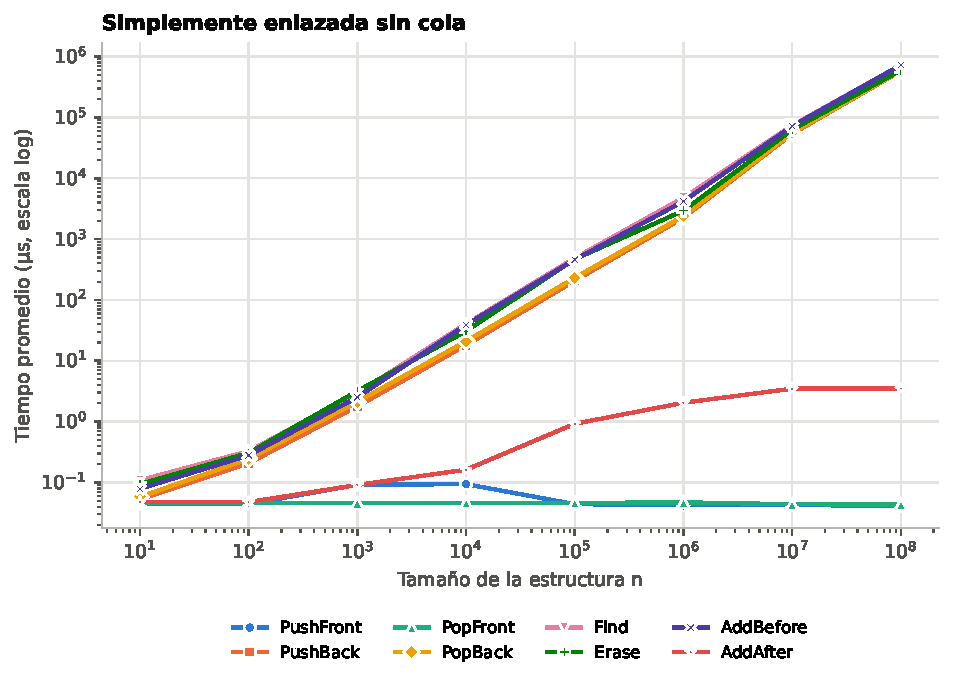
\includegraphics[width=0.86\linewidth]{figuras/lista_SLL_sin_cola.pdf}
\caption{Lista simplemente enlazada sin cola.}\label{fig:sll}
\end{figure}

\tablatiempos{lista_SLL_con_cola.tex}{Lista simplemente enlazada \textbf{con cola}: tiempo promedio (µs).\label{tab:sllt}}
\begin{figure}[H]\centering
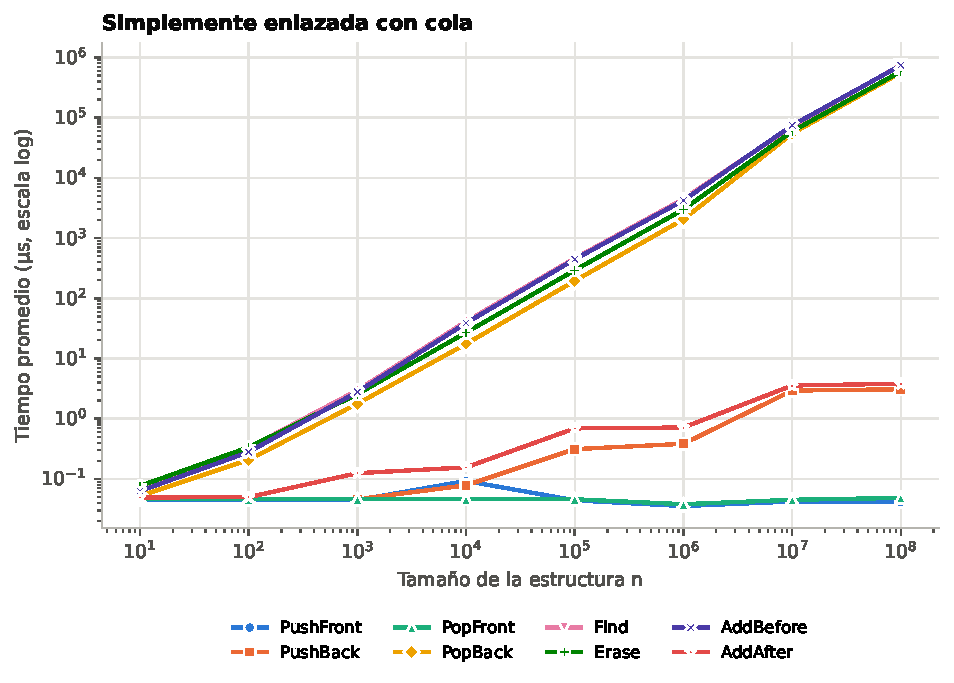
\includegraphics[width=0.86\linewidth]{figuras/lista_SLL_con_cola.pdf}
\caption{Lista simplemente enlazada con cola.}\label{fig:sllt}
\end{figure}

\tablatiempos{lista_DLL_sin_cola.tex}{Lista doblemente enlazada \textbf{sin cola}: tiempo promedio (µs).\label{tab:dll}}
\begin{figure}[H]\centering
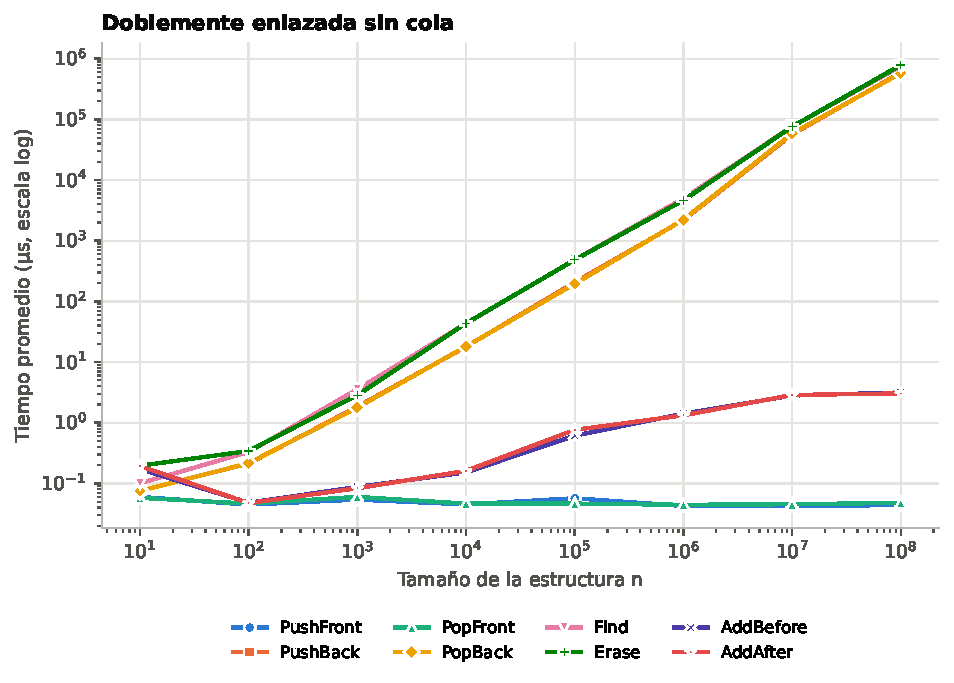
\includegraphics[width=0.86\linewidth]{figuras/lista_DLL_sin_cola.pdf}
\caption{Lista doblemente enlazada sin cola.}\label{fig:dll}
\end{figure}

\tablatiempos{lista_DLL_con_cola.tex}{Lista doblemente enlazada \textbf{con cola}: tiempo promedio (µs).\label{tab:dllt}}
\begin{figure}[H]\centering
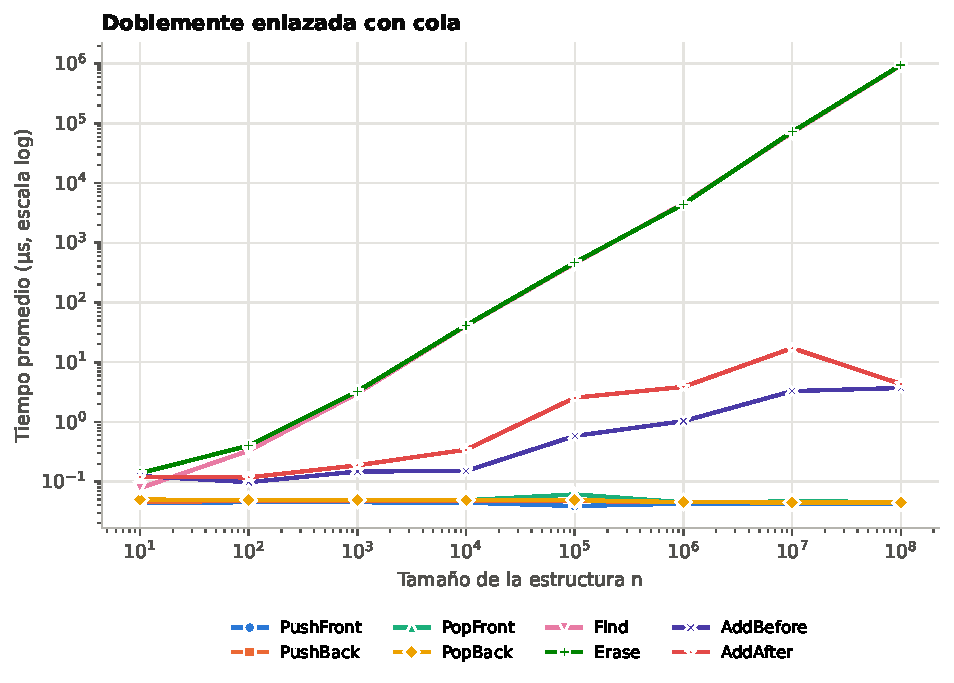
\includegraphics[width=0.86\linewidth]{figuras/lista_DLL_con_cola.pdf}
\caption{Lista doblemente enlazada con cola.}\label{fig:dllt}
\end{figure}

\begin{table}[H]\centering\small
\caption{Métodos auxiliares (\texttt{TopFront}, \texttt{TopBack}, \texttt{Empty}, \texttt{Size}) de las cuatro listas, µs.}
\resizebox{0.49\linewidth}{!}{\begin{tabular}{crrrr}
\toprule
$n$ & \textbf{TopFront} & \textbf{TopBack} & \textbf{Empty} & \textbf{Size} \\
\midrule
$10^{1}$ & 0{,}051 & 0{,}059 & 0{,}051 & 0{,}052 \\
$10^{2}$ & 0{,}052 & 0{,}215 & 0{,}052 & 0{,}053 \\
$10^{3}$ & 0{,}052 & 1{,}801 & 0{,}052 & 0{,}057 \\
$10^{4}$ & 0{,}052 & 17{,}7 & 0{,}052 & 0{,}056 \\
$10^{5}$ & 0{,}068 & 210{,}8 & 0{,}052 & 0{,}054 \\
$10^{6}$ & 0{,}052 & 2\,102 & 0{,}052 & 0{,}055 \\
$10^{7}$ & 0{,}049 & 55\,605 & 0{,}049 & 0{,}050 \\
$10^{8}$ & 0{,}050 & 565\,734 & 0{,}064 & 0{,}068 \\
\midrule
Teórico & $O(1)$ & $O(n)$ & $O(1)$ & $O(1)$ \\
Razón $\times 10$ & $\times$1{,}0 & $\times$10{,}2 & $\times$1{,}3 & $\times$1{,}4 \\
Empírico & $O(1)$ & $O(n)$ & $O(1)$ & $O(1)$ \\
\bottomrule
\end{tabular}}\hfill
\resizebox{0.49\linewidth}{!}{\begin{tabular}{crrrr}
\toprule
$n$ & \textbf{TopFront} & \textbf{TopBack} & \textbf{Empty} & \textbf{Size} \\
\midrule
$10^{1}$ & 0{,}052 & 0{,}052 & 0{,}052 & 0{,}053 \\
$10^{2}$ & 0{,}052 & 0{,}052 & 0{,}052 & 0{,}053 \\
$10^{3}$ & 0{,}052 & 0{,}052 & 0{,}052 & 0{,}057 \\
$10^{4}$ & 0{,}052 & 0{,}052 & 0{,}052 & 0{,}057 \\
$10^{5}$ & 0{,}052 & 0{,}052 & 0{,}051 & 0{,}053 \\
$10^{6}$ & 0{,}043 & 0{,}043 & 0{,}043 & 0{,}044 \\
$10^{7}$ & 0{,}050 & 0{,}050 & 0{,}050 & 0{,}050 \\
$10^{8}$ & 0{,}051 & 0{,}050 & 0{,}054 & 0{,}055 \\
\midrule
Teórico & $O(1)$ & $O(1)$ & $O(1)$ & $O(1)$ \\
Razón $\times 10$ & $\times$1{,}0 & $\times$1{,}0 & $\times$1{,}1 & $\times$1{,}1 \\
Empírico & $O(1)$ & $O(1)$ & $O(1)$ & $O(1)$ \\
\bottomrule
\end{tabular}}\\[3pt]
{\footnotesize Simple sin cola \hspace{5.2cm} Simple con cola}\\[6pt]
\resizebox{0.49\linewidth}{!}{\begin{tabular}{crrrr}
\toprule
$n$ & \textbf{TopFront} & \textbf{TopBack} & \textbf{Empty} & \textbf{Size} \\
\midrule
$10^{1}$ & 0{,}058 & 0{,}074 & 0{,}088 & 0{,}060 \\
$10^{2}$ & 0{,}052 & 0{,}217 & 0{,}052 & 0{,}053 \\
$10^{3}$ & 0{,}051 & 1{,}776 & 0{,}051 & 0{,}057 \\
$10^{4}$ & 0{,}052 & 17{,}7 & 0{,}052 & 0{,}057 \\
$10^{5}$ & 0{,}057 & 206{,}8 & 0{,}052 & 0{,}054 \\
$10^{6}$ & 0{,}052 & 2\,161 & 0{,}049 & 0{,}050 \\
$10^{7}$ & 0{,}050 & 58\,277 & 0{,}049 & 0{,}050 \\
$10^{8}$ & 0{,}050 & 583\,623 & 0{,}052 & 0{,}051 \\
\midrule
Teórico & $O(1)$ & $O(n)$ & $O(1)$ & $O(1)$ \\
Razón $\times 10$ & $\times$1{,}0 & $\times$10{,}0 & $\times$1{,}1 & $\times$1{,}0 \\
Empírico & $O(1)$ & $O(n)$ & $O(1)$ & $O(1)$ \\
\bottomrule
\end{tabular}}\hfill
\resizebox{0.49\linewidth}{!}{\begin{tabular}{crrrr}
\toprule
$n$ & \textbf{TopFront} & \textbf{TopBack} & \textbf{Empty} & \textbf{Size} \\
\midrule
$10^{1}$ & 0{,}052 & 0{,}052 & 0{,}077 & 0{,}053 \\
$10^{2}$ & 0{,}052 & 0{,}052 & 0{,}076 & 0{,}053 \\
$10^{3}$ & 0{,}052 & 0{,}052 & 0{,}076 & 0{,}057 \\
$10^{4}$ & 0{,}052 & 0{,}052 & 0{,}058 & 0{,}057 \\
$10^{5}$ & 0{,}052 & 0{,}052 & 0{,}052 & 0{,}053 \\
$10^{6}$ & 0{,}050 & 0{,}050 & 0{,}049 & 0{,}050 \\
$10^{7}$ & 0{,}050 & 0{,}050 & 0{,}049 & 0{,}049 \\
$10^{8}$ & 0{,}050 & 0{,}051 & 0{,}054 & 0{,}051 \\
\midrule
Teórico & $O(1)$ & $O(1)$ & $O(1)$ & $O(1)$ \\
Razón $\times 10$ & $\times$1{,}0 & $\times$1{,}0 & $\times$1{,}1 & $\times$1{,}0 \\
Empírico & $O(1)$ & $O(1)$ & $O(1)$ & $O(1)$ \\
\bottomrule
\end{tabular}}\\[3pt]
{\footnotesize Doble sin cola \hspace{5.4cm} Doble con cola}
\end{table}

\begin{figure}[H]\centering
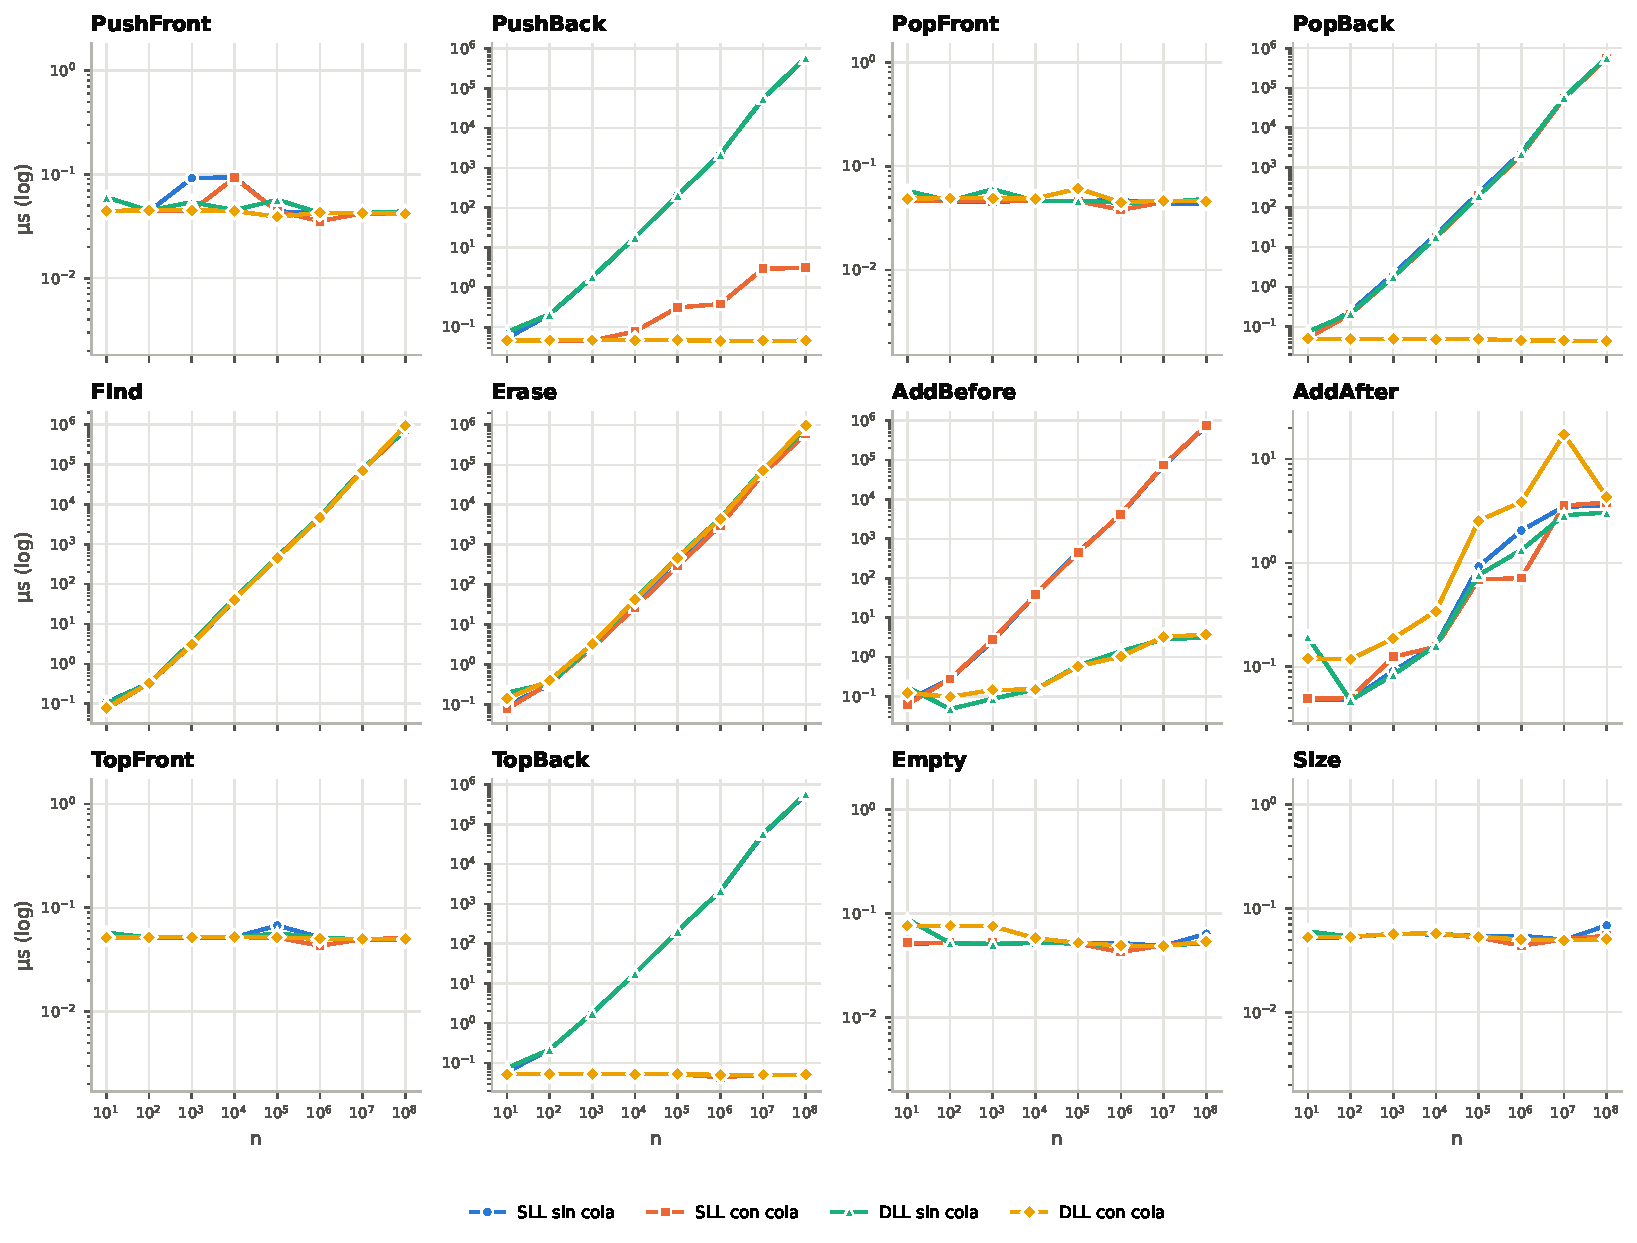
\includegraphics[width=\linewidth]{figuras/lista_por_metodo.pdf}
\caption{Cada método comparado entre las cuatro implementaciones.}\label{fig:pormetodo}
\end{figure}

\paragraph{Teórico vs. empírico.} En las cuatro implementaciones y los doce métodos, la clasificación
empírica coincide con la teórica. Todos los métodos \On{} multiplican su tiempo por
$\approx10$ entre $10^7$ y $10^8$ (razones entre $\times9{,}5$ y $\times13{,}4$), y todos los \Oone{}
se mantienen prácticamente constantes. Los casos más ilustrativos:
\begin{itemize}
\item \textbf{PopBack} es el método que mejor separa las variantes. Sin cola, o con cola pero simple,
  vale 0,56--0,59\,s para $10^8$ elementos; en la doble con cola vale 0,044\us: unos \textbf{13 millones
  de veces menos}, y constante desde $n=10$. Esto confirma la explicación de la sección 2: a la lista
  simple con cola no le basta con \texttt{tail}, le hace falta \texttt{prev}.
\item \textbf{PushBack} y \textbf{TopBack} pasan de \On{} a \Oone{} en cuanto la lista guarda
  \texttt{tail}, sea simple o doble.
\item \textbf{AddBefore} separa simples de dobles, sin importar la cola: 0,73--0,74\,s en las simples
  contra 3--4\us{} en las dobles para $n=10^8$.
\item \textbf{Find} y \textbf{Erase} son \On{} en las cuatro, como se esperaba: guardar \texttt{tail}
  o \texttt{prev} no ayuda a encontrar un valor arbitrario.
\end{itemize}

\paragraph{Efectos que no son de complejidad.} Dos fenómenos aparecen en las gráficas y conviene
explicarlos para no confundirlos con Big-O:
\begin{enumerate}
\item \emph{Salto entre $10^6$ y $10^7$.} Los métodos \On{} se multiplican por entre $\times15$ y $\times27$ en esa
  década, y no por 10. Con $10^6$ nodos (unos 24\,MB) la lista todavía cabe en buena parte en la memoria
  caché del procesador; con $10^7$ (unos 240\,MB) ya no, y cada salto a \texttt{next} puede esperar a
  la memoria RAM, que es mucho más lenta. Entre $10^7$ y $10^8$ la lista ya no cabe en ningún caso y el
  crecimiento vuelve a ser $\times10$. Es un cambio en la \emph{constante} (de 2--5\,ns a
  6--9\,ns por nodo recorrido), no en la complejidad.
\item \emph{Algunos métodos \Oone{} suben hasta $\approx3$\us{} y luego se estabilizan.} Es el caso de
  \texttt{AddAfter}/\texttt{AddBefore} en las dobles y de \texttt{PushBack} en la simple con cola.
  Justo antes de medirlos, la preparación o el deshacer de la repetición anterior recorren la lista
  entera (el \texttt{find} para obtener el nodo, el \texttt{popBack} \On{} que deshace el
  \texttt{pushBack}). Ese recorrido saca de la caché todo lo que la operación medida necesita, que
  entonces sufre unos pocos fallos de caché: un costo fijo de unos microsegundos. La prueba de que es
  constante es la última década: de $10^7$ a $10^8$ esos métodos cambian entre $\times0{,}25$ y $\times1{,}13$,
  mientras que un método \On{} cambiaría $\times10$. La doble con cola en \texttt{PushBack}, cuyo
  deshacer es \Oone{} y no ensucia la caché, se mantiene plana en 0,046\us.
\end{enumerate}

\paragraph{Constantes entre variantes (H1).} Entre implementaciones con la misma Big-O las
diferencias son pequeñas. En los métodos \Oone{} son de pocos nanosegundos y quedan por debajo de la
resolución (figura~\ref{fig:pormetodo}, paneles PushFront, PopFront, TopFront). En los métodos \On{},
como \texttt{Find}, varían hasta un 30\,\% para $n=10^8$ (0,72\,s en la simple sin cola frente a
0,94\,s en la doble con cola). Esa diferencia depende de cómo quedaron los nodos en memoria y no de la
estructura del algoritmo: en la JVM usada (64 bits con referencias comprimidas) un nodo simple ocupa
20 bytes que se redondean a 24, y uno doble exactamente 24, así que ambos ocupan lo mismo. La H1 se
confirma.

% ---------------------------------------------------------------------------
\subsection{Parte 2: MyStack y MyQueue con arreglo circular}
% ---------------------------------------------------------------------------

\tablatiemposcorta{pila.tex}{\texttt{ArrayStack} (implementa \texttt{MyStack}): tiempo promedio (µs).\label{tab:pila}}
\begin{figure}[H]\centering
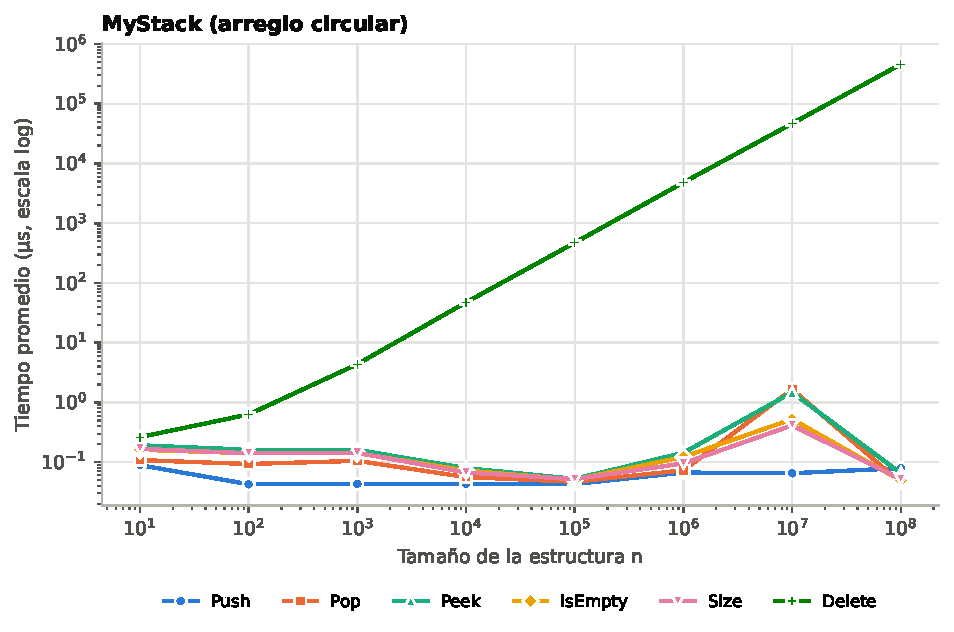
\includegraphics[width=0.84\linewidth]{figuras/pilacola_ArrayStack.pdf}
\caption{Métodos de la pila sobre arreglo circular dinámico.}\label{fig:pila}
\end{figure}

\tablatiemposcorta{cola.tex}{\texttt{ArrayQueue} (implementa \texttt{MyQueue}): tiempo promedio (µs).\label{tab:cola}}
\begin{figure}[H]\centering
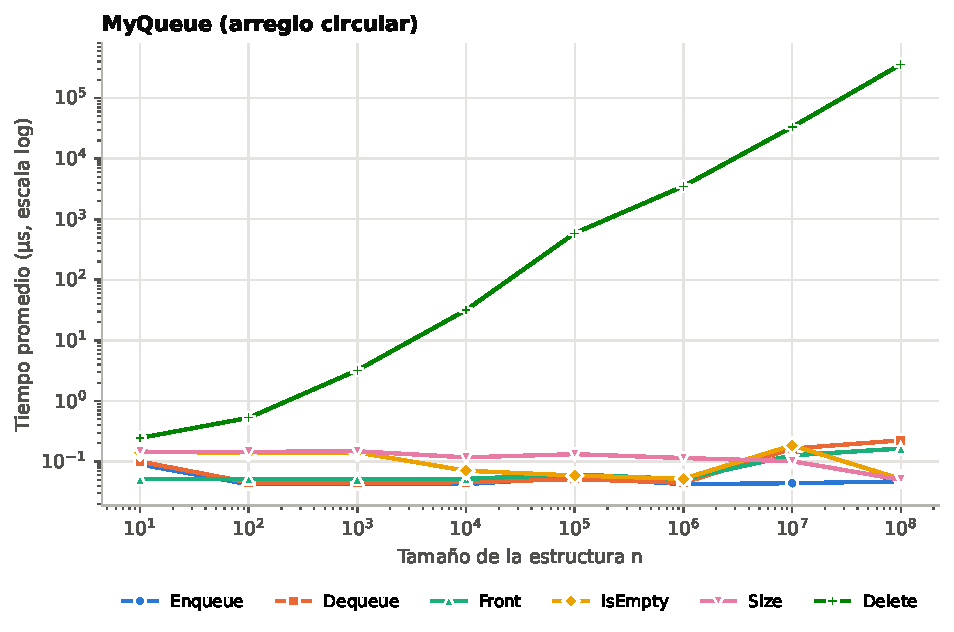
\includegraphics[width=0.84\linewidth]{figuras/pilacola_ArrayQueue.pdf}
\caption{Métodos de la cola sobre arreglo circular dinámico.}\label{fig:cola}
\end{figure}

\paragraph{Teórico vs. empírico.} De nuevo coinciden. \texttt{push}, \texttt{pop}, \texttt{peek},
\texttt{enqueue}, \texttt{dequeue}, \texttt{front}, \texttt{isEmpty} y \texttt{size} se mantienen entre
0,04 y 0,22\us{} de $n=10$ a $n=10^8$ (salvo un pico aislado en $10^7$, comentado abajo): \Oone. \texttt{delete} crece exactamente $\times10$ por década
($\times9{,}8$ en la pila, $\times10{,}8$ en la cola): \On. En $n=10^7$ varios métodos \Oone{} de la pila
muestran un pico aislado de 0,4--1,7\us{}. No se repite en $10^8$, así que corresponde a interferencia
puntual del sistema (con solo 10 repeticiones en ese tamaño, una pausa pesa en el promedio), no a
crecimiento.

\texttt{delete} en la pila (0,46\,s para $10^8$) es un 27\,\% más lento que en la cola (0,36\,s). Esto
concuerda con los casos medidos: en la pila el valor está en la base, así que se recorren los $n$
elementos \emph{y además} se desplazan $n-1$; en la cola el valor está al final y solo se recorre. En
ambos casos el trabajo es proporcional a $n$.

\subsubsection{Análisis del crecimiento del arreglo dinámico}\label{sec:crecimiento}

Para analizar la estrategia de crecimiento se hicieron dos experimentos adicionales (tabla~\ref{tab:crec}
y figura~\ref{fig:crec}):
\begin{enumerate}
\item \textbf{Costo total de $n$ inserciones} desde una pila vacía de capacidad 8, dividido entre $n$.
  Con la estrategia de \textbf{duplicar} el costo por inserción se mantiene entre 4,5 y 6\,ns desde
  $n=10^3$ hasta $n=10^8$: es \Oone{} amortizado, como predice el análisis de la sección 2.3. Este
  número es además la mejor estimación del costo real de un \texttt{push}, sin el piso de 40--70\,ns
  que impone medir operaciones sueltas. Con \textbf{incremento fijo de +1000} el costo por inserción
  crece con $n$ y el total se multiplica por $\times98$ entre $10^5$ y $10^6$ (cuadrático). Para
  $n=10^6$ tarda 424\,ms, \textbf{95 veces más} que duplicando (4,5\,ms). Para $10^7$ tardaría varios
  minutos, así que no se midió. Se confirma la H3.
\item \textbf{Un solo push con el arreglo lleno.} Es la inserción que dispara la copia. Crece
  linealmente con $n$ y llega a 163\,ms para $n=10^8$, frente a 0,08\us{} de un \texttt{push} normal.
  Esta es la otra cara del costo amortizado: el promedio es excelente, pero una operación puntual puede
  ser millones de veces más lenta que las demás.
\end{enumerate}

\begin{table}[H]\centering\small
\caption{Inserción de $n$ elementos desde vacío: tiempo total y costo por inserción según la estrategia de crecimiento.}\label{tab:crec}
\begin{tabular}{crrrr}
\toprule
$n$ & \textbf{x2: total} & \textbf{x2: ns/push} & \textbf{+1000: total} & \textbf{+1000: ns/push} \\
\midrule
$10^{1}$ & 0{,}132 µs & 13{,}2 & 0{,}760 µs & 76{,}0 \\
$10^{2}$ & 0{,}616 µs & 6{,}2 & 1{,}061 µs & 10{,}6 \\
$10^{3}$ & 4{,}677 µs & 4{,}7 & 3{,}445 µs & 3{,}4 \\
$10^{4}$ & 50{,}8 µs & 5{,}1 & 69{,}0 µs & 6{,}9 \\
$10^{5}$ & 450{,}4 µs & 4{,}5 & 4\,303 µs & 43{,}0 \\
$10^{6}$ & 4\,459 µs & 4{,}5 & 423\,563 µs & 423{,}6 \\
$10^{7}$ & 52\,721 µs & 5{,}3 & -- & -- \\
$10^{8}$ & 587\,541 µs & 5{,}9 & -- & -- \\
\bottomrule
\end{tabular}
\end{table}
\begin{figure}[H]\centering
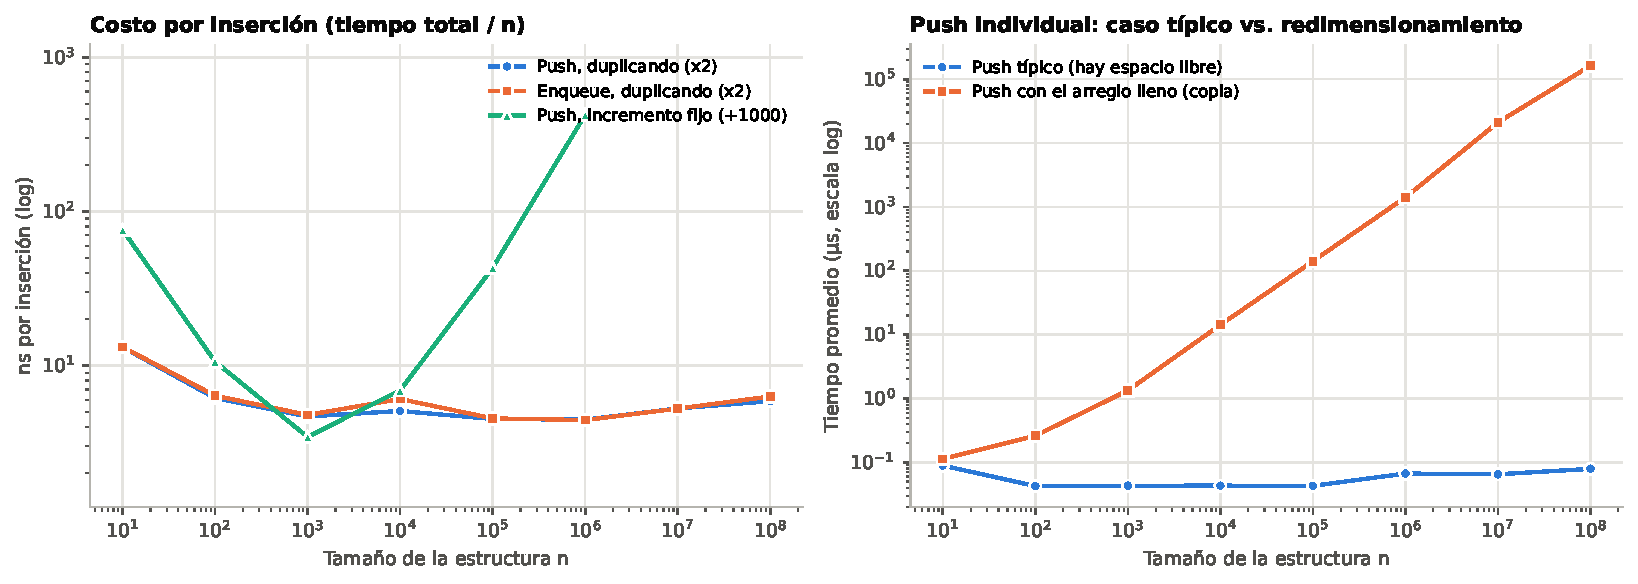
\includegraphics[width=\linewidth]{figuras/crecimiento.pdf}
\caption{Izquierda: costo amortizado por inserción (duplicar vs. incremento fijo). Derecha: \texttt{push} típico vs. \texttt{push} con el arreglo lleno.}\label{fig:crec}
\end{figure}

% ---------------------------------------------------------------------------
\subsection{Parte 3: comparativa de métodos equivalentes List / (Stack, Queue)}
% ---------------------------------------------------------------------------

Una pila se puede implementar con una lista usando solo el inicio: \texttt{push} = \texttt{pushFront},
\texttt{pop} = \texttt{popFront}, \texttt{peek} = \texttt{topFront}. Una cola, insertando al final y
sacando del inicio: \texttt{enqueue} = \texttt{pushBack}, \texttt{dequeue} = \texttt{popFront},
\texttt{front} = \texttt{topFront}. Además, \texttt{delete} equivale a \texttt{erase}, e
\texttt{isEmpty}/\texttt{size} a \texttt{Empty}/\texttt{Size}.

\paragraph{Criterio para elegir la implementación de List.} Para cada método se eligió la variante más
óptima en dos pasos: (1) la de \textbf{mejor complejidad teórica}; (2) entre las empatadas, la
\textbf{más liviana}, es decir, la que mantiene menos referencias por operación (simple antes que doble,
sin cola antes que con cola cuando la cola no se usa). El paso (2) no se basa en los tiempos medidos
porque, como mostró la parte 1, las variantes empatadas difieren en pocos nanosegundos, por debajo de
la resolución, y elegir por ese ruido no tendría sentido.

\begin{itemize}
\item \textbf{PushFront, PopFront, TopFront} (vs. \texttt{push}, \texttt{pop}, \texttt{peek},
  \texttt{dequeue}, \texttt{front}): son \Oone{} en las cuatro variantes. Se elige la \textbf{simple sin
  cola}, porque en cada operación solo actualiza \texttt{head}. Las otras tres, además, tendrían que
  mantener \texttt{tail} o \texttt{prev}, que una pila no necesita.
\item \textbf{PushBack} (vs. \texttt{enqueue}): solo las variantes con cola son \Oone. Entre ellas se
  elige la \textbf{simple con cola}: es la mínima estructura que da una cola eficiente
  (\texttt{pushBack} \Oone{} por \texttt{tail}, \texttt{popFront} \Oone{} por \texttt{head}), y no
  necesita \texttt{prev} porque una cola nunca saca por el final.
\item \textbf{Erase} (vs. \texttt{delete}): es \On{} en las cuatro. Se elige la \textbf{simple sin
  cola}, la más sencilla.
\item \textbf{Empty, Size}: \Oone{} en todas gracias al contador; \textbf{simple sin cola}.
\end{itemize}

\begin{table}[H]\centering\small
\caption{Métodos equivalentes: implementación de lista elegida y tiempo para $n=10^8$.}\label{tab:equiv}
\resizebox{\linewidth}{!}{\begin{tabular}{llllrr}
\toprule
\textbf{Lista} & \textbf{Implementación elegida} & \textbf{Arreglo circular} & \textbf{Big-O (L / A)} & \textbf{Lista (µs)} & \textbf{Arreglo (µs)} \\
\midrule
PushFront & SLL sin cola & ArrayStack.Push & $O(1)$ / $O(1)^{*}$ & 0{,}041 & 0{,}079 \\
PopFront & SLL sin cola & ArrayStack.Pop & $O(1)$ / $O(1)$ & 0{,}043 & 0{,}045 \\
TopFront & SLL sin cola & ArrayStack.Peek & $O(1)$ / $O(1)$ & 0{,}050 & 0{,}065 \\
PushBack & SLL con cola & ArrayQueue.Enqueue & $O(1)$ / $O(1)^{*}$ & 3{,}087 & 0{,}047 \\
PopFront & SLL sin cola & ArrayQueue.Dequeue & $O(1)$ / $O(1)$ & 0{,}043 & 0{,}224 \\
TopFront & SLL sin cola & ArrayQueue.Front & $O(1)$ / $O(1)$ & 0{,}050 & 0{,}164 \\
Erase & SLL sin cola & ArrayStack.Delete & $O(n)$ / $O(n)$ & 595\,694 & 459\,725 \\
Erase & SLL sin cola & ArrayQueue.Delete & $O(n)$ / $O(n)$ & 595\,694 & 360\,588 \\
Empty & SLL sin cola & ArrayStack.IsEmpty & $O(1)$ / $O(1)$ & 0{,}064 & 0{,}049 \\
Size & SLL sin cola & ArrayStack.Size & $O(1)$ / $O(1)$ & 0{,}068 & 0{,}052 \\
\bottomrule
\end{tabular}}
\end{table}
\begin{figure}[H]\centering
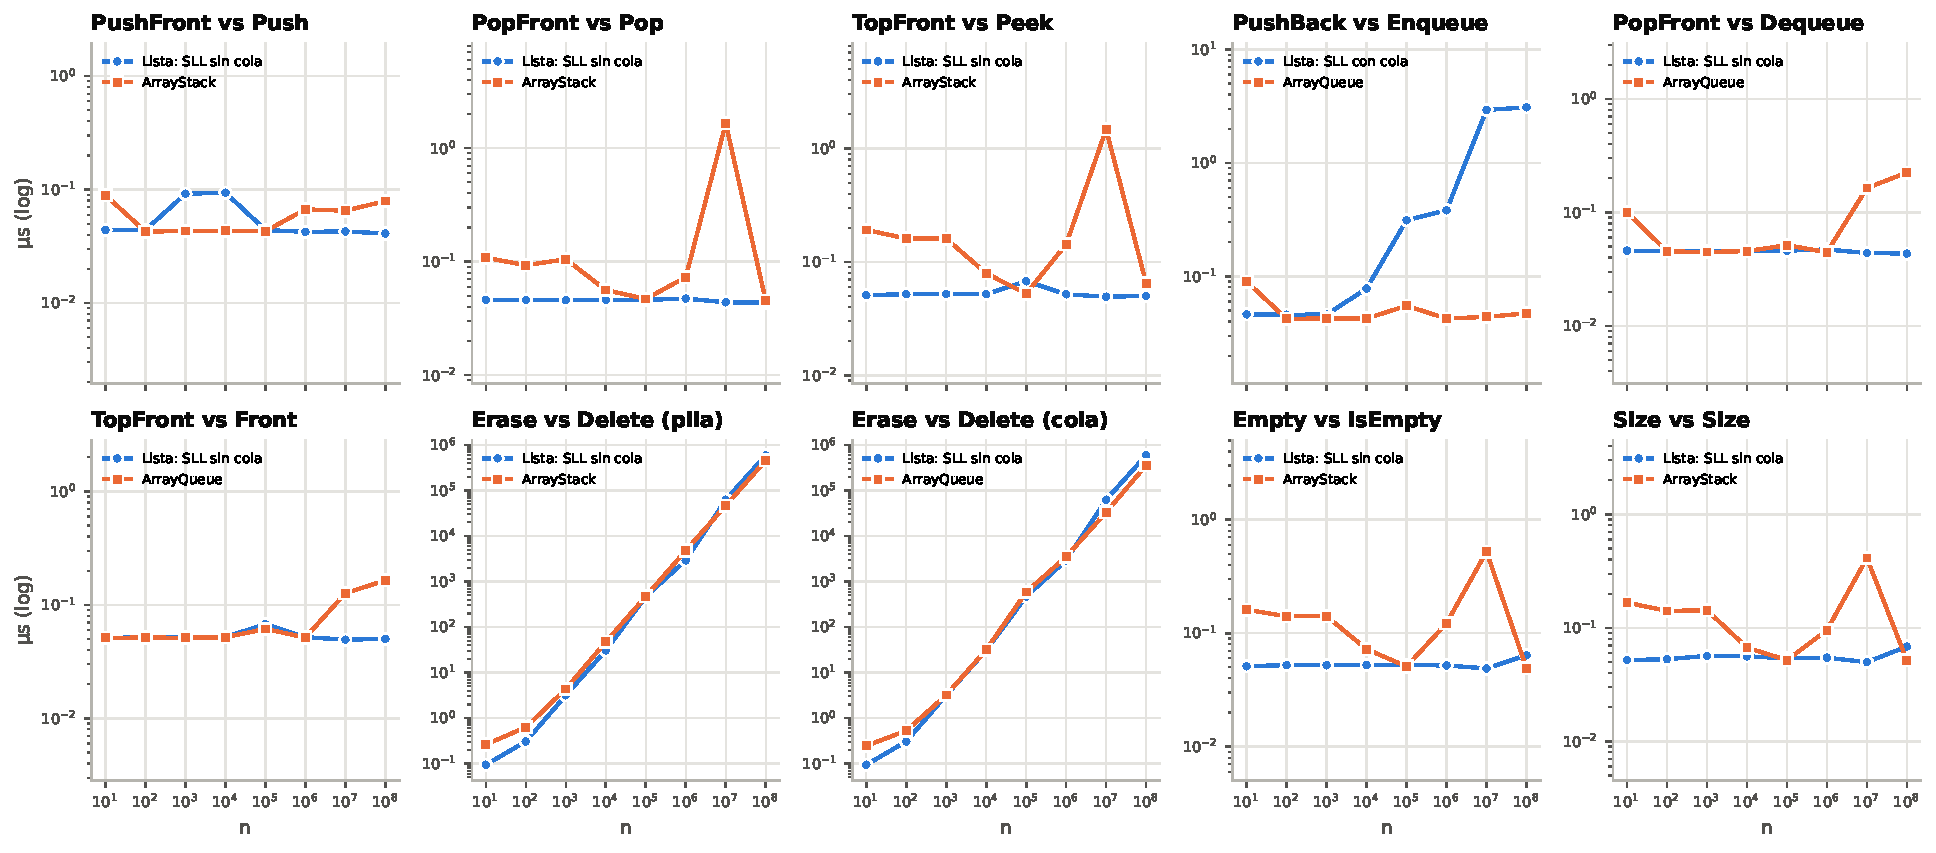
\includegraphics[width=\linewidth]{figuras/comparativa_equivalentes.pdf}
\caption{Lista (implementación elegida) vs. arreglo circular, método por método.}\label{fig:equiv}
\end{figure}

\paragraph{Resultados.}
\begin{itemize}
\item \textbf{Operaciones \Oone{} (push/pop/peek, dequeue/front, isEmpty/size):} empatan. Ambas
  estructuras quedan en 0,04--0,2\us{} en todo el rango, sin tendencia (salvo el pico aislado de la
  pila en $10^7$). Con la resolución disponible no
  se puede declarar un ganador: las dos cumplen \Oone{} y la diferencia real es de unos pocos
  nanosegundos.
\item \textbf{PushBack vs. enqueue:} ambos son \Oone{} y ambos quedan planos en la última década. La
  lista marca $\approx3$\us{} para $n \ge 10^7$ por el efecto de caché explicado en la parte 1: su
  deshacer (\texttt{popBack} \On) ensucia la caché antes de cada medición. Aun así hay una diferencia
  estructural real. Cada \texttt{pushBack} crea un objeto nodo nuevo, que el recolector de basura
  tendrá que gestionar, mientras que \texttt{enqueue} escribe una referencia en una posición ya
  reservada del arreglo.
\item \textbf{Erase vs. delete:} los tres son \On{} y sus curvas son paralelas (figura~\ref{fig:equiv}).
  Para $n$ pequeño la lista es algo más rápida, porque \texttt{delete} además desplaza elementos. Para
  $n$ grande el arreglo gana a pesar de hacer más trabajo: para $n=10^8$, 0,46\,s en la pila (que
  recorre y desplaza) y 0,36\,s en la cola, frente a 0,60\,s en la lista. Por elemento, el arreglo
  procesa $\approx3{,}6$\,ns en la cola (solo búsqueda) y la lista $\approx6$\,ns por nodo. El arreglo
  es memoria contigua que el procesador lee por bloques y anticipa; la lista obliga a seguir una
  referencia a una posición arbitraria por cada nodo. Se confirma la H2.
\end{itemize}

% ===========================================================================
\section{Conclusiones}
% ===========================================================================

\subsection{Cuándo usar cada estructura}
\begin{itemize}
\item \textbf{Lista simple sin cola:} cuando solo se opera por un extremo, es decir, como pila o como
  lista que se recorre de principio a fin. Es la más liviana en código y en referencias por nodo.
\item \textbf{Lista simple con cola:} cuando se inserta por el final y se saca por el inicio (cola
  FIFO). Si también se necesita sacar por el final, no sirve: \texttt{popBack} sigue siendo \On.
\item \textbf{Lista doble sin cola:} poco útil por sí sola. Paga el costo de mantener \texttt{prev} y
  solo gana \texttt{addBefore} \Oone, pero sigue siendo \On{} en todo lo que ocurre al final.
\item \textbf{Lista doble con cola:} la única con todas las operaciones de los extremos en \Oone{}
  (sirve como \emph{deque}) y con inserción y eliminación \Oone{} en cualquier punto del que ya se
  tenga la referencia. Es la opción cuando se insertan o borran elementos en medio de una secuencia,
  por ejemplo en listas de reproducción, editores de texto o una caché LRU (lista doble más tabla hash).
\item \textbf{Pila y cola con arreglo circular dinámico:} la mejor opción general para pilas y colas.
  Tienen la misma complejidad que la mejor lista, pero usan mucha menos memoria (4 a 8 bytes por
  elemento contra 24 de un nodo), no crean objetos por cada inserción y recorren más rápido por la
  localidad de memoria. Su debilidad es la latencia puntual al crecer (163\,ms para $10^8$). Si el
  tamaño máximo se conoce de antemano, se evita reservando la capacidad desde el constructor.
\item \textbf{Nunca} conviene hacer crecer un arreglo dinámico en una cantidad fija: convierte $n$
  inserciones en $O(n^2)$.
\end{itemize}

\subsection{Pilas y colas en aplicaciones reales}
\begin{itemize}
\item \textbf{Pilas (LIFO):} la pila de llamadas de cualquier programa (cada llamada a un método apila
  su contexto y el \texttt{return} lo desapila; por eso la recursión infinita causa
  \texttt{StackOverflowError}); deshacer/rehacer en editores; el botón ``atrás'' del navegador;
  verificación de paréntesis balanceados y evaluación de expresiones en compiladores y calculadoras;
  recorrido en profundidad (DFS) y \emph{backtracking}, como en laberintos o sudokus.
\item \textbf{Colas (FIFO):} colas de impresión y de tareas en sistemas operativos; atención de
  solicitudes en servidores web y \emph{pools} de hilos; colas de mensajes entre servicios; búferes de
  audio y video en \emph{streaming}, donde el arreglo circular de tamaño fijo es precisamente la
  estructura estándar (\emph{ring buffer}); recorrido en anchura (BFS), por ejemplo para calcular la
  ruta con menos transbordos en un sistema de transporte.
\end{itemize}

\subsection{Arreglos dinámicos vs. listas enlazadas en Java}
\begin{table}[H]\centering\small
\begin{tabular}{p{3.6cm} p{5.6cm} p{5.6cm}}
\toprule
 & \textbf{Arreglo dinámico} & \textbf{Lista enlazada} \\
\midrule
Acceso por posición & \Oone{} & \On{} \\
Insertar/borrar en extremos & \Oone{} amortizado (con arreglo circular) & \Oone{} (con cola y, para \texttt{popBack}, doble) \\
Insertar/borrar en medio & \On{} (desplazar) & \Oone{} si ya se tiene el nodo \\
Memoria por elemento & 4--8 bytes (referencia más espacio libre) & 24 bytes por nodo más la referencia \\
Recorrido & Rápido: memoria contigua, caché & Lento: un salto de memoria por nodo \\
Recolector de basura & Un solo objeto grande & Un objeto por elemento \\
Peor caso puntual & Copia \On{} al crecer & Estable, sin picos por crecimiento \\
\bottomrule
\end{tabular}
\end{table}

En la práctica, en Java el arreglo dinámico gana en la gran mayoría de los casos. Por la misma razón,
la documentación de Java recomienda \texttt{ArrayDeque} (un arreglo circular dinámico, como el de este
trabajo) antes que \texttt{LinkedList} para implementar pilas y colas. La lista enlazada se justifica
cuando hay muchas inserciones o eliminaciones en medio de la secuencia a partir de referencias ya
conocidas, o cuando no se pueden tolerar los picos de latencia de un redimensionamiento.

La lección más general del trabajo es que Big-O predijo correctamente cómo \emph{escala} cada
método, en los 60 casos medidos, pero no dice nada de las \emph{constantes}. La memoria caché, el
recolector de basura y la resolución del reloj cambiaron los tiempos por factores de 2 a 25 sin alterar
la clase de complejidad. Para decidir entre dos estructuras con la misma Big-O hay que medir, y medir
bien: una sola operación a la vez, en el peor caso, con calentamiento, repeticiones y sin mezclar la
medición con otras tareas.

\end{document}
